\documentclass[a4paper,12pt]{article}
\usepackage[utf8]{inputenc}
\usepackage{amsmath}
\usepackage{booktabs}
\usepackage{geometry}
\geometry{margin=1in}
\usepackage{graphicx}


\title{Analysis of Dermatology Data}
\author{}
\date{}

\begin{document}

\maketitle

\section{Introduction}

\subsection{Context}
This study is based on a dermatological dataset obtained from the "Center for Machine Learning and Intelligent Systems" at the University of California, Irvine (UCI). The primary objective is to identify correlations between clinical and histopathological features and their association with different types of skin diseases.

The differential diagnosis of erythemato-squamous diseases is a significant challenge in dermatology. These diseases share common clinical features such as erythema and scaling, with subtle differences among them. The diseases included in this dataset are:
\begin{itemize}
    \item Psoriasis
    \item Seborrheic Dermatitis
    \item Lichen Planus
    \item Pityriasis Rosea
    \item Chronic Dermatitis
    \item Pityriasis Rubra Pilaris
\end{itemize}

Typically, a biopsy is required to distinguish between these diseases. However, histopathological analyses often reveal overlapping features, further complicating the diagnostic process. Moreover, diseases may initially exhibit the features of another disease during their early stages, before developing their characteristic features later on.

\subsection{Dataset Information}
The dataset comprises 34 attributes:
\begin{itemize}
    \item \textbf{Clinical attributes:} 12 features evaluated during clinical examinations.
    \item \textbf{Histopathological attributes:} 22 features determined through microscopic analysis of skin samples.
    \item \textbf{Class labels:} Six categories representing different skin diseases.
\end{itemize}

Each feature is rated on a scale from 0 to 3, where:
\begin{itemize}
    \item 0 indicates the absence of the feature.
    \item 3 indicates the highest intensity of the feature.
    \item Intermediate values (1 and 2) represent relative intensities.
\end{itemize}
The `family history` feature is binary (0 or 1), and the `age` feature is linear.

\subsection{Problem Statement}
This study aims to address the following questions:
\begin{enumerate}
    \item Are there significant correlations between clinical and the type of skin disease?
    \item Which variables play a key role in distinguishing between different skin disease classes?
\end{enumerate}

\subsection{Dataset Summary}
A summary of the dataset's structure is provided below:

\begin{table}[h!]
\centering
\begin{tabular}{ll}
\toprule
\textbf{Attribute Group}       & \textbf{Description} \\
\midrule
Clinical attributes            & 12 features rated on a scale of 0--3 \\
Histopathological attributes   & 22 features rated on a scale of 0--3 \\
Class labels                   & Six disease types \\
\bottomrule
\end{tabular}
\caption{Overview of dataset attributes.}
\end{table}

\subsection{Class Distribution}
The class distribution in the dataset is as follows:

\begin{table}[h!]
\centering
\begin{tabular}{llc}
\toprule
\textbf{Class Code} & \textbf{Disease}                  & \textbf{Number of Instances} \\
\midrule
1                  & Psoriasis                         & 112 \\
2                  & Seborrheic Dermatitis             & 61  \\
3                  & Lichen Planus                     & 72  \\
4                  & Pityriasis Rosea                  & 49  \\
5                  & Chronic Dermatitis                & 52  \\
6                  & Pityriasis Rubra Pilaris          & 20  \\
\bottomrule
\end{tabular}
\caption{Class distribution of skin diseases in the dataset.}
\end{table}

\section{Objective}
The primary objective of this study is to uncover significant relationships between the clinical and classify skin diseases accurately. This is achieved through:
\begin{itemize}
    \item Exploratory data analysis and descriptive statistics.
    \item Multivariate techniques such as Principal Component Analysis (PCA).
    \item Statistical hypothesis testing (e.g., Kruskal-Wallis test, post-hoc analysis).
\end{itemize}

\section{Data and Methodology}

\subsection{Origin of the Data}
The data originates from a dermatological study aimed at differentiating between six types of erythemato-squamous diseases. These diseases are characterized by overlapping clinical features such as erythema and scaling, making their diagnosis challenging. 

The dataset includes the following components:
\begin{itemize}
    \item \textbf{Clinical variables:} Observations directly assessed by medical professionals, such as erythema intensity and itching etc...
    \item \textbf{Target variable (Class):} Represents the type of skin disease, categorized into six classes.
\end{itemize}

For this study, we focus exclusively on the clinical variables and exclude histopathological features.

\subsection{Structure of the Data}
The dataset contains:
\begin{itemize}
    \item \textbf{Number of observations:} $366$ .
    \item \textbf{Number of variables:} $11$ (clinical features only).
\end{itemize}

A subset of the data structure is summarized below:

\begin{table}[h!]
\centering
\begin{tabular}{lll}
\toprule
\textbf{Variable} & \textbf{Type} & \textbf{Description} \\
\midrule
erythema          & Quantitative  & Intensity of erythema \\
scaling           & Quantitative  & Presence of scaling \\
itching           & Quantitative  & Presence of itching \\
koebner\_phenomenon & Quantitative & Koebner phenomenon occurrence \\
polygonal\_papules & Quantitative & Presence of polygonal papules \\
oral\_mucosal\_involvement & Quantitative & Oral mucosal involvement \\
knee\_and\_elbow\_involvement & Quantitative & Knee and elbow involvement \\
family\_history   & Binary        & Family history of similar conditions (0/1) \\
age               & Quantitative  & Age of the patient \\
Class             & Target        & Type of skin disease (1 to 6) \\
\bottomrule
\end{tabular}
\caption{Subset of the dataset structure.}
\end{table}

\subsection{Methodology}
To analyze the data and address the research questions, the following steps were undertaken:
\begin{enumerate}
    \item \textbf{Descriptive analysis:} To explore the distribution of clinical variables and the target class. This includes visualizing the frequency of diseases and summarizing variable statistics.
    \item \textbf{Multivariate analysis:} Principal Component Analysis (PCA) was applied to identify patterns and relationships between clinical variables and skin disease types.
    \item \textbf{Statistical tests:} 
    \begin{itemize} 
        \item Anova test to check if the data follows a normal distribution.
        \item Kruskal-Wallis tests were used to examine the significance of differences in clinical variables across disease classes.
        \item Post-hoc Dunn’s tests were conducted to pinpoint specific group differences for significant variables.
    \end{itemize}
\end{enumerate}

\subsection{Exclusions}
Histopathological attributes were excluded from this analysis, as the focus was strictly on clinical observations.

\section{Descriptive Analysis}

\subsection{Univariate Analysis}

\subsubsection{Distribution of Variables}

The histograms and boxplots presented below illustrate the distribution of the clinical variables. For instance, the variable \texttt{erythema} shows a heterogeneous distribution, with values concentrated around the mean.

% Histogram for erythema
\begin{figure}[h!]
\centering
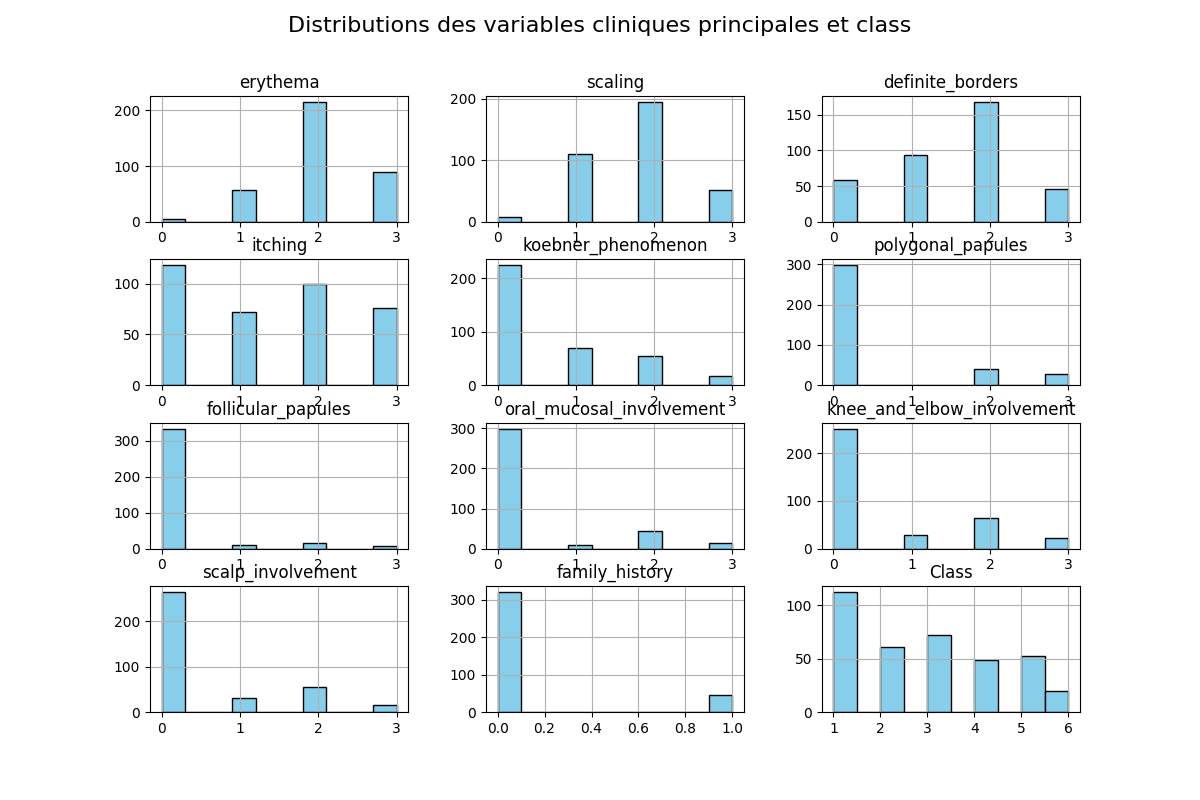
\includegraphics[width=0.8\textwidth]{Distributions_variables_cliniques_class.png}
\caption{Histogram of the \texttt{erythema} variable. The distribution shows a concentration of values around the mean, indicating heterogeneity.}
\end{figure}

% Boxplot for erythema
\begin{figure}[h!]
\centering
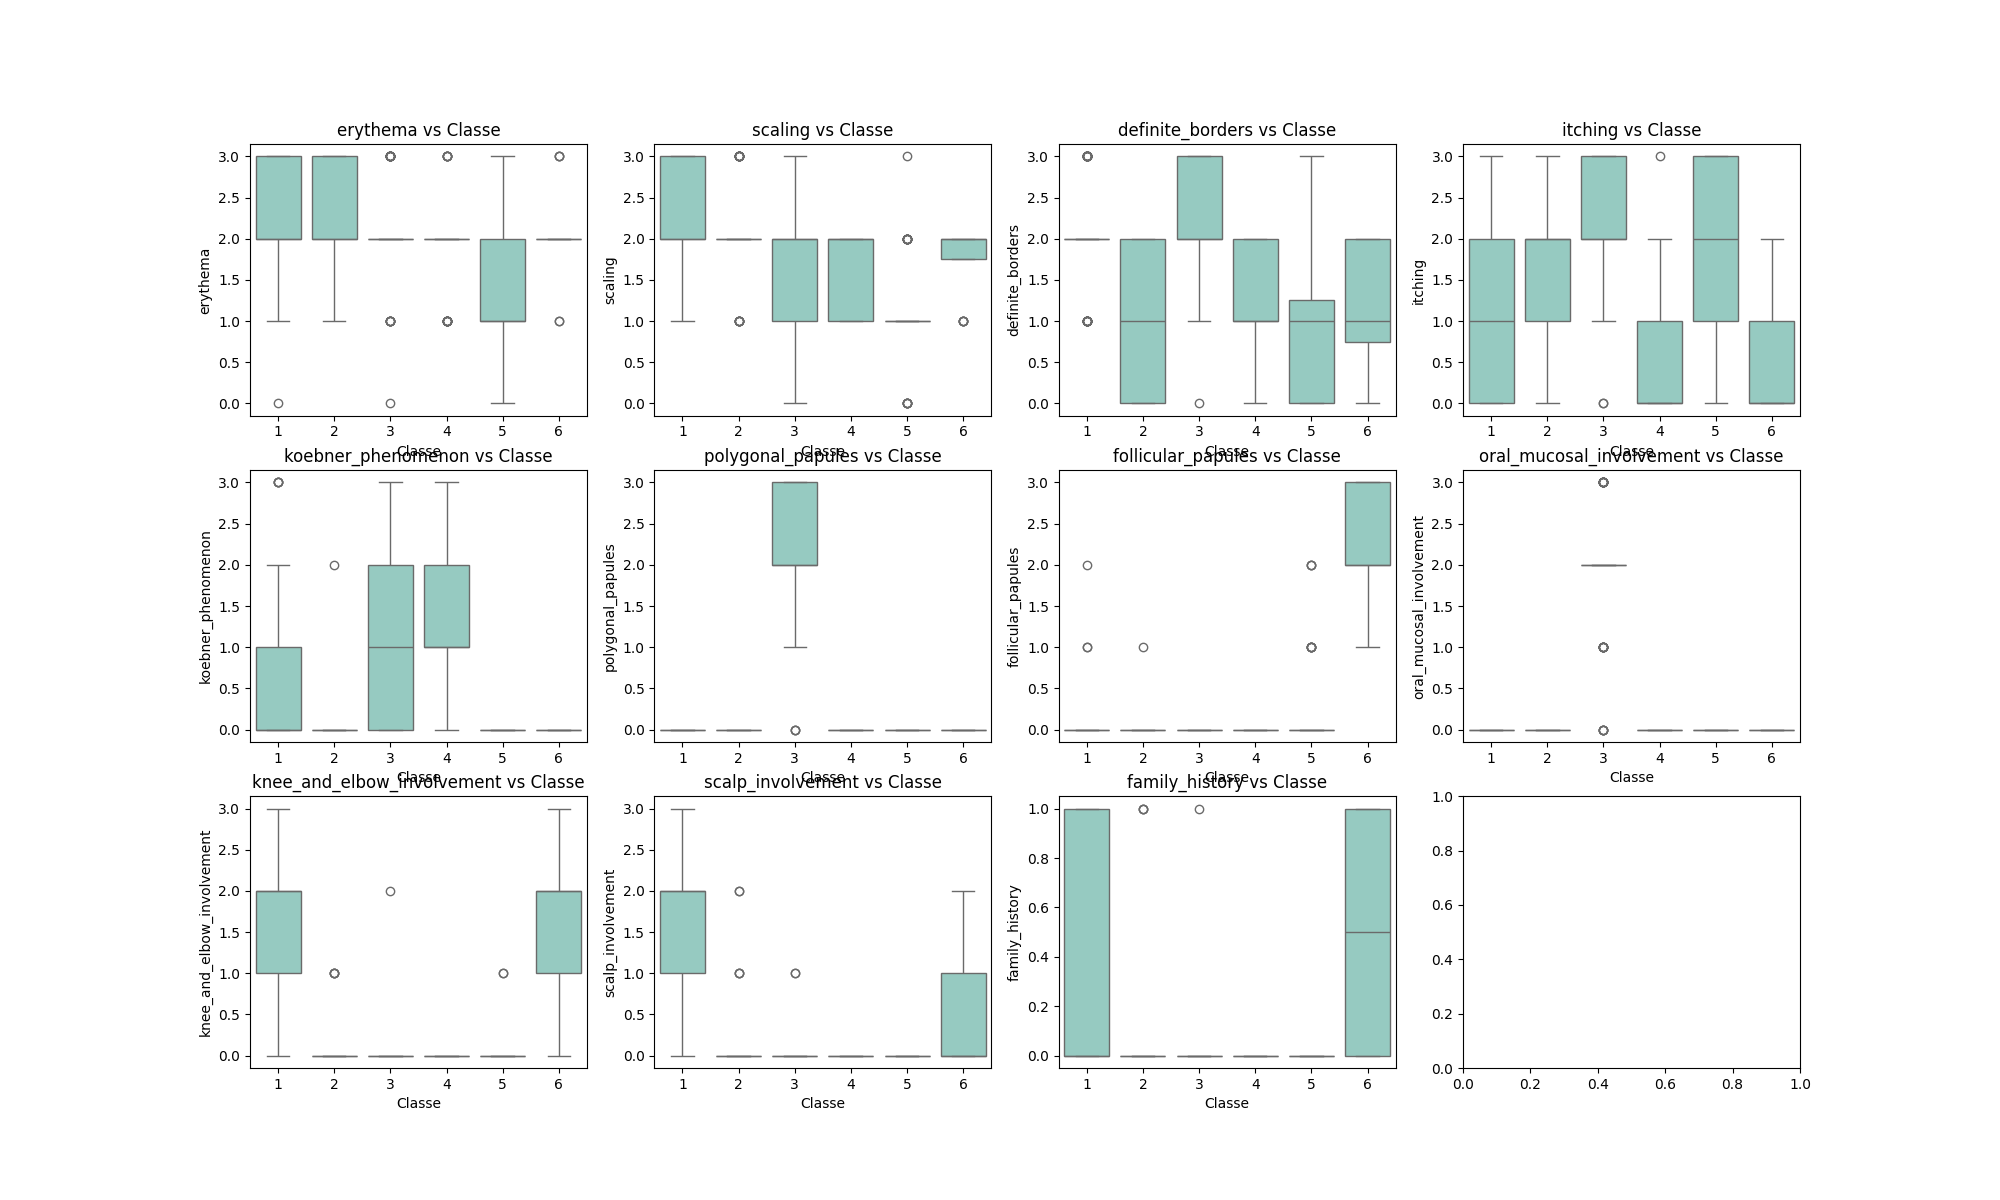
\includegraphics[width=0.8\textwidth]{boxplot_distribution.png}
\caption{Boxplot of the \texttt{erythema} variable. The plot shows the spread of values and the presence of outliers.}
\end{figure}

\subsubsection{Distribution of Classes}

The bar chart below indicates an imbalance in the distribution of the disease classes. This could affect the model’s ability to classify minority classes accurately.

% Barplot for Class distribution
\begin{figure}[h!]
\centering
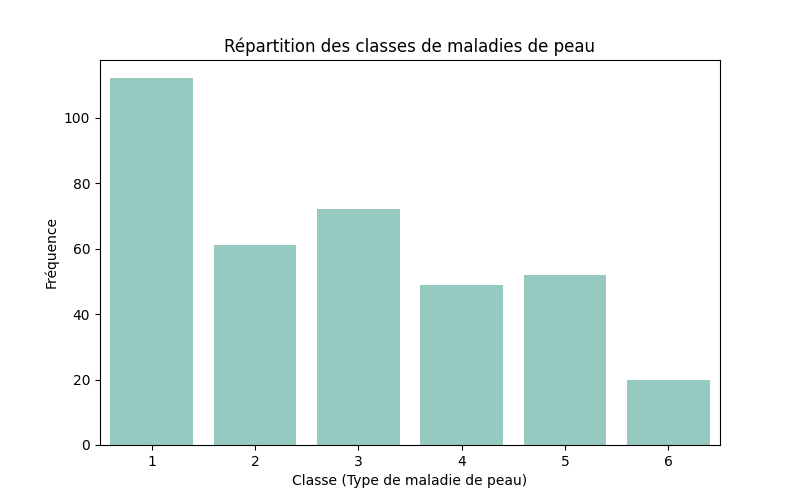
\includegraphics[width=0.8\textwidth]{Repartition_classes.png}
\caption{Bar plot showing the distribution of the disease classes. The dataset is imbalanced, with psoriasis being the most common disease.}
\end{figure}

\subsection{Bivariate Analysis}

\subsubsection{Correlations}

The correlation matrix below presents the relationships between the quantitative clinical variables. For example, the correlation between \texttt{scaling} and \texttt{erythema} is relatively weak, suggesting that these variables do not move in sync across all observations.

% Correlation matrix
\begin{figure}[h!]
\centering
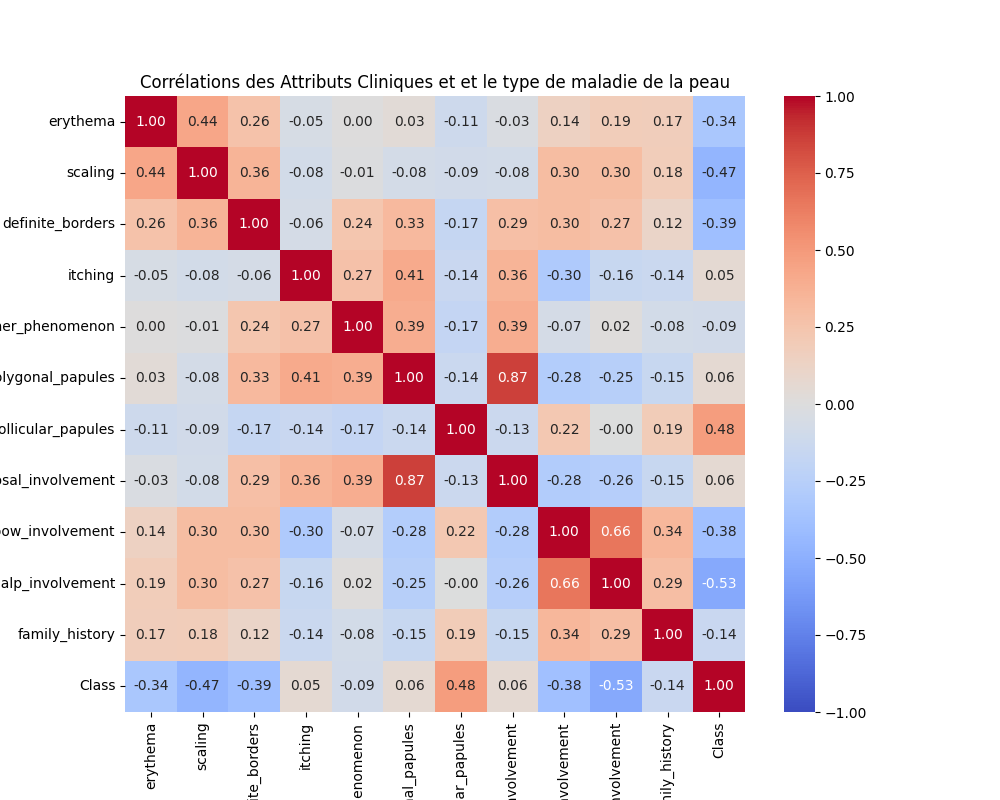
\includegraphics[width=0.8\textwidth]{correlation_matrix.png}
\caption{Correlation matrix of the clinical variables. The matrix reveals weak correlations between \texttt{scaling} and \texttt{erythema}.}
\end{figure}

%\subsubsection{Relations with Class}

%Boxplots below illustrate the differences in clinical variables across disease %classes. For example, there are significant differences between the classes in %terms of the \texttt{scaling} and \texttt{itching} variables.

% Boxplots showing relationships with Class (e.g., scaling vs. Class)
%\begin{figure}[h!]
%\centering
%\includegraphics[width=0.8\textwidth]{path/to/scaling_class_boxplot.png}
%\caption{Boxplot showing the distribution of \texttt{scaling} across different %disease classes. Significant differences are observed between classes.}
%\end{figure}

% Boxplot for another variable (e.g., itching vs. Class)
%\begin{figure}[h!]
%\centering
%\includegraphics[width=0.8\textwidth]{path/to/itching_class_boxplot.png}
%\caption{Boxplot showing the distribution of \texttt{itching} across disease %classes. A significant variation in the distribution of \texttt{itching} across %classes is observed.}%\end{figure}



\end{document}
